\documentclass[10pt]{article}
\usepackage[T1]{fontenc}

% Document Details
\newcommand{\CLASS}{AMATH 515}
\newcommand{\assigmentnum}{Problem Set 2}

\usepackage[margin = 1.5in]{geometry}
\usepackage{titling}
\setlength{\droptitle}{-6em}   % This is your set screw
\date{}
\renewcommand{\maketitle}{
	\clearpage
	\begingroup  
	\centering
	\LARGE \sffamily\textbf{\CLASS} \Large \assigmentnum\\[.8em]
	\large Tyler Chen\\[1em]
	\endgroup
	\thispagestyle{empty}
}
 % Title Styling


\usepackage{enumitem}

% Figures
\usepackage{subcaption}

% TikZ and Graphics
\usepackage{tikz, pgfplots}
\pgfplotsset{compat=1.12}
\usetikzlibrary{patterns,arrows}
\usepgfplotslibrary{fillbetween}

\usepackage{pdfpages}
\usepackage{adjustbox}

\usepackage{lscape}
\usepackage{titling}
\usepackage[]{hyperref}


% Header Styling
\usepackage{fancyhdr}
\pagestyle{fancy}
\lhead{\sffamily \CLASS}
\rhead{\sffamily Chen \textbf{\thepage}}
\cfoot{}

% Paragraph Styling
\setlength{\columnsep}{1cm}
\setlength{\parindent}{0pt}
\setlength{\parskip}{5pt}
\renewcommand{\baselinestretch}{1}

% TOC Styling
\usepackage{tocloft}
\iffalse
\renewcommand{\cftsecleader}{\cftdotfill{\cftdotsep}}

\renewcommand\cftchapafterpnum{\vskip6pt}
\renewcommand\cftsecafterpnum{\vskip10pt}
\renewcommand\cftsubsecafterpnum{\vskip6pt}

% Adjust sectional unit title fonts in ToC
\renewcommand{\cftchapfont}{\sffamily}
\renewcommand{\cftsecfont}{\bfseries\sffamily}
\renewcommand{\cftsecnumwidth}{2em}
\renewcommand{\cftsubsecfont}{\sffamily}
\renewcommand{\cfttoctitlefont}{\hfill\bfseries\sffamily\MakeUppercase}
\renewcommand{\cftaftertoctitle}{\hfill}

\renewcommand{\cftchappagefont}{\sffamily}
\renewcommand{\cftsecpagefont}{\bfseries\sffamily}
\renewcommand{\cftsubsecpagefont}{\sffamily}
\fi
 % General Styling
% Code Display Setup
\usepackage{listings,lstautogobble}
\usepackage{lipsum}
\usepackage{courier}
\usepackage{catchfilebetweentags}

\lstset{
	basicstyle=\small\ttfamily,
	breaklines=true, 
	frame = single,
	rangeprefix=,
	rangesuffix=,
	includerangemarker=false,
	autogobble = true
}


\usepackage{algorithmicx}
\usepackage{algpseudocode}

\newcommand{\To}{\textbf{to}~}
\newcommand{\DownTo}{\textbf{downto}~}
\renewcommand{\algorithmicdo}{\hspace{-.2em}\textbf{:}}
 % Code Display Setup
% AMS MATH Styling
\usepackage{amsmath, amssymb}
\newcommand{\qed}{\hfill\(\square\)}

%\newtheorem*{lemma}{Lemma} 
%\newtheorem*{theorem}{Theorem}
%\newtheorem*{definition}{Definition}
%\newtheorem*{prop}{Proposition}
%\renewenvironment{proof}{{\bfseries Proof.}}{}


% mathcal
\newcommand{\cA}{\ensuremath{\mathcal{A}}}
\newcommand{\cB}{\ensuremath{\mathcal{B}}}
\newcommand{\cC}{\ensuremath{\mathcal{C}}}
\newcommand{\cD}{\ensuremath{\mathcal{D}}}
\newcommand{\cE}{\ensuremath{\mathcal{E}}}
\newcommand{\cF}{\ensuremath{\mathcal{F}}}
\newcommand{\cG}{\ensuremath{\mathcal{G}}}
\newcommand{\cH}{\ensuremath{\mathcal{H}}}
\newcommand{\cI}{\ensuremath{\mathcal{I}}}
\newcommand{\cJ}{\ensuremath{\mathcal{J}}}
\newcommand{\cK}{\ensuremath{\mathcal{K}}}
\newcommand{\cL}{\ensuremath{\mathcal{L}}}
\newcommand{\cM}{\ensuremath{\mathcal{M}}}
\newcommand{\cN}{\ensuremath{\mathcal{N}}}
\newcommand{\cO}{\ensuremath{\mathcal{O}}}
\newcommand{\cP}{\ensuremath{\mathcal{P}}}
\newcommand{\cQ}{\ensuremath{\mathcal{Q}}}
\newcommand{\cR}{\ensuremath{\mathcal{R}}}
\newcommand{\cS}{\ensuremath{\mathcal{S}}}
\newcommand{\cT}{\ensuremath{\mathcal{T}}}
\newcommand{\cU}{\ensuremath{\mathcal{U}}}
\newcommand{\cV}{\ensuremath{\mathcal{V}}}
\newcommand{\cW}{\ensuremath{\mathcal{W}}}
\newcommand{\cX}{\ensuremath{\mathcal{X}}}
\newcommand{\cY}{\ensuremath{\mathcal{Y}}}
\newcommand{\cZ}{\ensuremath{\mathcal{Z}}}

% mathbb
\usepackage{bbm}
\newcommand{\bOne}{\ensuremath{\mathbbm{1}}}

\newcommand{\bA}{\ensuremath{\mathbb{A}}}
\newcommand{\bB}{\ensuremath{\mathbb{B}}}
\newcommand{\bC}{\ensuremath{\mathbb{C}}}
\newcommand{\bD}{\ensuremath{\mathbb{D}}}
\newcommand{\bE}{\ensuremath{\mathbb{E}}}
\newcommand{\bF}{\ensuremath{\mathbb{F}}}
\newcommand{\bG}{\ensuremath{\mathbb{G}}}
\newcommand{\bH}{\ensuremath{\mathbb{H}}}
\newcommand{\bI}{\ensuremath{\mathbb{I}}}
\newcommand{\bJ}{\ensuremath{\mathbb{J}}}
\newcommand{\bK}{\ensuremath{\mathbb{K}}}
\newcommand{\bL}{\ensuremath{\mathbb{L}}}
\newcommand{\bM}{\ensuremath{\mathbb{M}}}
\newcommand{\bN}{\ensuremath{\mathbb{N}}}
\newcommand{\bO}{\ensuremath{\mathbb{O}}}
\newcommand{\bP}{\ensuremath{\mathbb{P}}}
\newcommand{\bQ}{\ensuremath{\mathbb{Q}}}
\newcommand{\bR}{\ensuremath{\mathbb{R}}}
\newcommand{\bS}{\ensuremath{\mathbb{S}}}
\newcommand{\bT}{\ensuremath{\mathbb{T}}}
\newcommand{\bU}{\ensuremath{\mathbb{U}}}
\newcommand{\bV}{\ensuremath{\mathbb{V}}}
\newcommand{\bW}{\ensuremath{\mathbb{W}}}
\newcommand{\bX}{\ensuremath{\mathbb{X}}}
\newcommand{\bY}{\ensuremath{\mathbb{Y}}}
\newcommand{\bZ}{\ensuremath{\mathbb{Z}}}

% alternative mathbb
\newcommand{\NN}{\ensuremath{\mathbb{N}}}
\newcommand{\RR}{\ensuremath{\mathbb{R}}}
\newcommand{\CC}{\ensuremath{\mathbb{C}}}
\newcommand{\ZZ}{\ensuremath{\mathbb{Z}}}
\newcommand{\EE}{\ensuremath{\mathbb{E}}}
\newcommand{\PP}{\ensuremath{\mathbb{P}}}
\newcommand{\VV}{\ensuremath{\mathbb{V}}}
\newcommand{\cov}{\ensuremath{\text{Co}\VV}}
% Math Commands

\newcommand{\st}{~\big|~}
\newcommand{\stt}{\text{ st. }}
\newcommand{\ift}{\text{ if }}
\newcommand{\thent}{\text{ then }}
\newcommand{\owt}{\text{ otherwise }}

\newcommand{\norm}[1]{\left\lVert#1\right\rVert}
\newcommand{\snorm}[1]{\lVert#1\rVert}
\newcommand{\ip}[1]{\ensuremath{\left\langle #1 \right\rangle}}
\newcommand{\pp}[3][]{\frac{\partial^{#1}#2}{\partial #3^{#1}}}
\newcommand{\dd}[3][]{\frac{\d^{#1}#2}{\d #3^{#1}}}
\renewcommand{\d}{\ensuremath{\mathrm{d}}}

\newcommand{\indep}{\rotatebox[origin=c]{90}{$\models$}}




 % Math shortcuts
\usepackage{mdframed}

\newenvironment{algorithm}[1][\@nil]
{\def\tmp{#1}%
\begin{mdframed}[
  frametitle={Algorithm. \ifx\tmp\@nnil  \else \normalfont (#1) \fi},
  linecolor=green!70,
  linewidth=1,
  topline=false,
  bottomline=false,
  rightline=false,
  rightmargin=.5cm
]}
{\end{mdframed}}

\newenvironment{method}[1][\@nil]
{
\def\tmp{#1}%
\begin{mdframed}[
  frametitle={Method. \ifx\tmp\@nnil  \else \normalfont (#1) \fi},
  linecolor=violet!70,
  linewidth=1,
  topline=false,
  bottomline=false,
  rightline=false,
  rightmargin=.5cm
]}
{\end{mdframed}}

\newenvironment{definition}[1][\@nil]
{\def\tmp{#1}%
\begin{mdframed}[
  frametitle={Definition. \ifx\tmp\@nnil  \else \normalfont (#1) \fi},
  linecolor=blue!70,
  linewidth=1,
  topline=false,
  bottomline=false,
  rightline=false,
  rightmargin=.5cm
]}
{\end{mdframed}}

\newenvironment{theorem}[1][\@nil]
{\def\tmp{#1}%
\begin{mdframed}[
  frametitle={Theorem. \ifx\tmp\@nnil  \else \normalfont (#1) \fi},
  linecolor=red!70,
  linewidth=1,
  topline=false,
  bottomline=false,
  rightline=false,
  rightmargin=.5cm
]}
{\end{mdframed}}

\newenvironment{lemma}[1][\@nil]
{\def\tmp{#1}%
\begin{mdframed}[
  frametitle={Lemma. \ifx\tmp\@nnil  \else \normalfont (#1) \fi},
  linecolor=red!70,
  linewidth=1,
  topline=false,
  bottomline=false,
  rightline=false,
  rightmargin=.5cm
]}
{\end{mdframed}}

\newenvironment{proof}[1][\@nil]
{\def\tmp{#1}%
\begin{mdframed}[
  frametitle={Proof. \ifx\tmp\@nnil  \else \normalfont (#1) \fi},
  linecolor=red!30,
  linewidth=1,
  topline=false,
  bottomline=false,
  rightline=false,
  rightmargin=.5cm
]}
{\end{mdframed}}



 % Proof shortcuts
% Problem
\usepackage{floatrow}

\newenvironment{problem}[1][]
{\pagebreak
\noindent\rule{\textwidth}{1pt}\vspace{0.25em}
{\sffamily \textbf{#1}}
\par
}
{\par\vspace{-0.5em}\noindent\rule{\textwidth}{1pt}}

\newenvironment{solution}[1][]
{{\sffamily \textbf{#1}}
\par
}
{}

 % Problem Environment

\rhead{\sffamily Tyler Chen \textbf{\thepage}}

\let\savedprob=\problem%
\def\problem[#1]{\pagebreak\phantomsection\addcontentsline{toc}{subsection}{#1}\savedprob[#1]\label{#1}\setcounter{page}{1}}

\newcommand{\sgn}{\operatorname{sgn}}
\newcommand{\rank}{\operatorname{rank}}
\newcommand{\range}{\operatorname{range}}
\newcommand{\prox}{\operatorname{prox}}
\DeclareMathOperator*{\proj}{\operatorname{proj}}

\usepackage{placeins}


\begin{document}
\maketitle


\begin{problem}[Problem 1]
    \begin{enumerate}[label=(\alph*)]
        \item[(a)] 	Show that a \( \mathcal{C}^1 \)-smooth function \( f \) is \( \alpha \)-strongly convex if and only if the function \( g(x) = f (x) - \frac{\alpha}{2} \|x\|^2 \) is convex.
\item[(b)] 	Suppose that \( f \) is \( \alpha \)-strongly convex. Show that any minimizer of \( f \) is unique. 
\item[(c)] 	Suppose that \( f \) is \( \alpha \)-strongly convex with minimizer \( x^* \). Show that 
\[
f(x) \geq f(x^*) + \frac{\alpha}{2} \|x-x^*\|^2. 
\]
\end{enumerate}

\end{problem}

\begin{solution}[Solution]
\begin{enumerate}[label=(\alph*)]
    \item 
        Observe that,
        \begin{align*}
            \nabla g(x) = \nabla f(x) - \alpha x
        \end{align*}

        Then we have the following equivalence,
        \begin{align*}
            && g(x) \text{ is convex}
            \\ \Longleftrightarrow &&
            \ip{ \nabla g(y) - \nabla g(x) , y-x } &\geq 0
            \\ \Longleftrightarrow &&
            \ip{ \nabla f(y) - \nabla f(x) - (\alpha y - \alpha x), y-x } &\geq 0
            \\ \Longleftrightarrow &&
            \ip{ \nabla f(y) - \nabla f(x) , y-x} - \alpha \ip{ y-x,y-x} &\geq 0
            \\ \Longleftrightarrow &&
            \ip{ \nabla f(y) - \nabla f(x) , y-x} - \alpha \norm{y-x}^2 &\geq 0
            \\ \Longleftrightarrow &&
            \ip{ \nabla f(y) - \nabla f(x) , y-x} &\geq \alpha \norm{y-x}^2
            \\ \Longleftrightarrow &&
            f(x) \text{ is \(\alpha\)-strictly convex} \tag*{\qed}
        \end{align*}
        
       
    \item Suppose \( x^* \) is a minimizer of \( f \). Then \( \nabla f(x^*) = 0 \) so,
        \begin{align*}
            f(x) \geq f(x^*) + \ip{\nabla f(x^*), x-x^*} + \frac{\alpha}{2} \norm{x-x^*}^2
            = f(x^*) + \frac{\alpha}{2} \norm{x-x^*}^2
        \end{align*}
        Therefore, for any \( \alpha > 0 \), \( f(x) = f(x^*) \) if and only if \( x = x^* \). That is, the minimizer \( x^* \) is unique. \qed
        
    \item This was shown as an intermediate step in the previous result. \qed


\end{enumerate}


\end{solution}

\begin{problem}[Problem 2]
Recall that 
\[
\begin{aligned}
\mbox{prox}_{t f}(y) &= \arg\min_{x} \frac{1}{2t}\|x-y\|^2 + f(x)\\
f_t(y) &= \min_x \frac{1}{2t}\|x-y\|^2 + f(x).
\end{aligned}
\] 
Suppose \( f \) is convex. 
\begin{enumerate}[label=(\alph*)]
%\item Prove \( \mbox{prox}_f(x) + \mbox{prox}_{f^*}(x) = x \).
\item Prove that \( f_t \) is convex.  
\item Prove that \( \prox_{t f} \) is a single-valued mapping. 
\item Compute \( \prox_{t f} \) and \( f_t \), where \( f(x) = \|x\|_1 \). 
%One way to do this is to consider the scalar case, and explicitly compute \( f'(t) \) 
%\[
%f'_t(x) = \frac{1}{t} (x-\prox_{t f}(x)).
%\]
%Now, just find a function that has this derivative. 
\item Compute \( \prox_{t f} \) and \( f_t \) for \( f = \delta_{\mathbb{B}_{\infty}}(x) \), 
where \( \mathbb{B}_\infty = [-1,1]^n \).
\end{enumerate}
\end{problem}

\begin{solution}[Solution]
\begin{enumerate}[label=(\alph*)]
    \item Assume \( f \) is convex. Recall that for a fixed \( x \), \( \norm{x-y}^2 \) is a convex function of \( y \). Therefore, for all \( x \), 
        \begin{align*}
            \norm{x-(\lambda y + (1-\lambda)z)}^2
            \leq \lambda \norm{x-y}^2 + (1-\lambda)\norm{x-z}^2
        \end{align*}

        Observe that for any \( x_1 \) and \( x_2 \), by the convexity of \( \norm{\cdot}^2 \), 
        \begin{align*}
            \norm{ \lambda x_1 + (1-\lambda)x_2 - (\lambda y + (1-\lambda)z)} ^2
            &= \norm{\lambda(x_1-y) + (1-\lambda)(x_2-z)}^2
            \\&\leq \lambda \norm{x_1-y}^2 + (1-\lambda)\norm{x_2-z}^2
        \end{align*}

        Similarly,
        \begin{align*}
            f(\lambda x_1 + (1-\lambda)x_2) \leq \lambda f(x_1) + (1-\lambda)f(x_2)
        \end{align*}
        
        Then, 
        \begin{align*}
            f_t(\lambda y + (1-\lambda)z)
            &= \min_x \left[ \frac{1}{2t} \norm{x-(\lambda y + (1-\lambda) z)}^2 + f(x) \right]
            %\\&\leq \min_x \left[ \frac{1}{2t} \left( \lambda \norm{x- y}^2 + (1-\lambda)\norm{x- z}^2 \right) + (\lambda + (1-\lambda))f(x) \right]
            \\&\leq \lambda \min_{x_1} \left[ \frac{1}{2t} \norm{x_1 - y}^2 + f(x) \right] + (1-\lambda) \min_{x_2} \left[\frac{1}{2t}\norm{x_2- z}^2 + f(x) \right]
            \\&= \lambda f_t(y) + (1-\lambda)f_t(z) %\tag*{\qed}
        \end{align*}
        where the inequality holds by observing that the convex combination of whichever \( x_1 \) and \( x_2 \) are used in the middle line provided an upper bound for the top line.

    \item Fix \( y \) and suppose \( x_1 \neq x_2 \) satisfy,
        \begin{align*}
            \frac{1}{2t} \norm{x_1-y}^2 + f(x_1) = \frac{1}{2t}\norm{x_2-y}^2 + f(x_2)
        \end{align*}

        Recall that \( \norm{x-y}^2 \) as a function of \( x \) is strictly convex. Therefore, the point \( x = (x_1 + x_2)/2 \) satisfies,
        \begin{align*}
            \frac{1}{2t} \norm{x-y}^2 + f(x) 
            &< \frac{1}{2} \left( \frac{1}{2t} \norm{x_1-y}^2 + f(x_1) \right) + \frac{1}{2} \left( \frac{1}{2t} \norm{x_2-y}^2 + f(x_2) \right)
            \\&= \frac{1}{2t} \norm{x_1-y}^2 + f(x_1)
            \\&= \frac{1}{2t} \norm{x_2-y}^2 + f(x_2)
        \end{align*}
        
        Therefore neither of \( x_1 \) and \( x_1 \) can be an output to \( \prox_{tf} \). \qed
        
    \item 
        By definition,
        \begin{align*}
            \prox_{tf}(y) 
            &= \arg\min_x \left[ \frac{1}{2t} \norm{x-y}^2 + \lambda\norm{x}_1 \right]
            \\&= \arg\min_x \left[ \sum_{i=1}^{n} \frac{1}{2t} (x_i-y_i)^2 + \lambda|x_i| \right]
        \end{align*}
       
        Now observe that the components are decoupled so that we only need to compute,
        \begin{align*}
            \arg\min_{x_i} \left[ \frac{1}{2t} (x_i-y_i)^2 + \lambda|x_i| \right]
        \end{align*}

        As a function of \( x_i \), the argument above, which we well denote \( h_i(x) \), is a quadratic centered at \( y_i \) plus an absolute value centered at 0.


        We consider three cases, \( y_i \in(-\infty, -\lambda t) \), \( y_i \in [-\lambda t, \lambda t] \), and \( y_i \in (\lambda t, \infty) \). For each of theses cases we consider \( x_i < 0 \), \( x_i > 0 \) and \( x_i = 0 \). 

        First, suppose \( y_i \in (-\infty, -\lambda t) \). If \( x_i \leq 0 \) then setting the derivative to zero we find \( x_i = y_i+\lambda t \) minimizes \( h_i \) and that \( h_i(y_i+\lambda t) = \lambda^2t/2+|y_i+\lambda t| \). If \( x_i > 0 \) then the derivative is nonzero so \( h_i \) is not minimized.

        Similarly, suppose \( y_i \in (\lambda t, \infty) \). If \( x_i \leq 0 \) then setting the derivative to zero we find \( x_i = y_i-\lambda t \) minimizes \( h_i \) and \( h_i(y_i-\lambda t) = \lambda^2t/2+|y_i-\lambda t| \). If \( x_i < 0 \) then the derivative is nonzero so \( h_i \) is not minimized.


       Finally, suppose \( y_i \in [- \lambda t, \lambda t] \). If \( x_i = 0 \) then the subgradient is \( y_i/t + [-\lambda,\lambda] \), so zero is in the subgradient exactly when \( |y_i| < \lambda t \). In this case, \( h_i(0) = y_i^2/2t \). If \( x_i \neq 0 \) then zero is not contained in the subgradient so \( h_i \) is not minimized.

        Therefore,
        \begin{align*}
            \left[\prox_{tf}(y) \right]_i
            = \arg\min_{x_i} \left[ \frac{1}{2t} (x_i-y_i)^2 + \lambda |x_i| \right]
            = \begin{cases}
                y_i+\lambda t, & y_i\in (-\infty, -\lambda t) \\
                0, & y_i\in[-\lambda t,\lambda t] \\
                y_i-\lambda t & y_i\in(\lambda t,\infty)
            \end{cases}
        \end{align*}
       
        Similarly,
        \begin{align*}
            f_t = \sum_{i} \left[ f_t \right]_t
        \end{align*}
        where
        \begin{align*}
            \left[ f_{t} \right]_i
            = \min_{x_i} \left[ \frac{1}{2t} (x_i-y_i)^2 + \lambda |x_i| \right]
            = \begin{cases}
                \frac{\lambda^2 t}{2} + |y_i+\lambda t|, & y_i\in (-\infty, -\lambda t) \\
                \frac{y_i^2}{2t}, & y_i\in[-\lambda t,\lambda t] \\
                \frac{\lambda^2 t}{2} + |y_i-\lambda t| & y_i\in(\lambda t,\infty)
        \end{cases}
        \end{align*}

        

    \item Note that for a fixed \( y \), \( \norm{x-y} \) is the distance from \( x \) to \( y \), which is minimized at \( y \). Then, the projection of \( y \) to some set minimizes this quantity over that set. Therefore,
        \begin{align*}
            \prox_{tf}(y) 
            &= \arg\min_x \left[ \frac{1}{2} \norm{x-y}^2 + \delta_{\bB_\infty}(x) \right]
            \\&= \arg\min_{x\in\bB_\infty} \frac{1}{2t}\norm{x-y}^2
            \\&= \proj_{\bB_\infty} y
            \\&= \min (\max( y, -1),1)
        \end{align*}
where \( \min \) and \( \max \) are taken pointwise.

    Then,
    \begin{align*}
        f_t = \frac{1}{2t}\left[\operatorname{dist}_{\bB_\infty} (y) \right]^2 = 
        \frac{1}{2t}\sum_{i} \left[f_t\right]_i
    \end{align*}
    where,
    \begin{align*}
        \left[ f_t \right]_i = 
        \begin{cases}
            (y_i+1)^2 & y_i\in(-\infty,-1) \\
            0 & y_i \in [-1,1] \\
            (y_i - 1)^2 & y_i \in(1,\infty)
        \end{cases}
    \end{align*}
    

\end{enumerate}

\end{solution}


\begin{problem}[Problem 3]
More prox identities. 
\vskip 16pt
\begin{enumerate}[label=(\alph*)]
%\item Prove \( \mbox{prox}_f(x) + \mbox{prox}_{f^*}(x) = x \).
\item Suppose \( f \) is convex and let \( g(x) = f(x) + \frac{1}{2}\|x-x_0\|^2 \). 
Find formulas for \( \prox_{t g} \) and \( g_t \) in terms of \( \prox_{t f} \) and \( f_t \).
\item The elastic net penalty is used to detect groups of correlated predictors:
\[
g(x) = \beta \|x\|_1 + (1-\beta) \frac{1}{2}\|x\|^2, \quad \beta \in (0,1).
\] 
Write down the formula for \( \prox_{t g} \) and \( g_t \).
\item Let \( f(x) = \frac{1}{2}\|Cx\|^2 \). Write \( \prox_{t f}(y) \) in closed form.
\item Let \( f(x) = \|x\|_2 \). Write \( \prox_{tf}(y) \) in closed form.
\end{enumerate}
\end{problem}

\begin{solution}[Solution]
\begin{enumerate}[label=(\alph*)]
    \item     
        By definition,
        \begin{align*}
            \prox_{tg}(y) 
            &= \arg\min_x \left[ \frac{1}{2t} \norm{x-y}^2 + g(x) \right]
            \\&= \arg\min_x \left[ \frac{1}{2t} \norm{x-y}^2 + f(x) + \frac{1}{2}\norm{x-x_0}^2 \right]
        \end{align*}
        
        Observe that by completing the square,
        \begin{align*}
            \norm{x-y}^2 + t\norm{x-x_0}^2
            = (1+t) \norm{x - \frac{y+tx_0}{1+t}}^2 
            + \frac{t}{1+t} \norm{y-x_0}^2
            %- \frac{\norm{y+tx_0}^2}{1+t} + \norm{y}^2 + t\norm{x_0}^2
        \end{align*}
        
        Thus, define,
        \begin{align*}
            s = \frac{t}{1+t}
            ,&&
            z = \frac{y+t x_0}{1+t}
        \end{align*}

        Then, observing that the last terms when completing the square to not affect \( \prox_{tg} \) as they depend only on \( y \) and \( x_0 \) but not \( x \), we find that,
        \begin{align*}
            \prox_{tg}(y) = \prox_{sf}(z)
        \end{align*}

        Similarly, by definition,
        \begin{align*}
            g_t(y) 
            &= \min_x \left[ \frac{1}{2t} \norm{x-y}^2 + g(x) \right]
            \\&= \min_x \left[ \frac{1}{2t} \norm{x-y}^2 + f(x) + \frac{1}{2}\norm{x-x_0}^2 \right]
        \end{align*}

        So, adding the difference term from \( f_s(z) \) and \( g_t(y) \) we find,
        \begin{align*}
            g_t(y) = f_s(z) + \frac{\norm{y-x}^2}{2(1+t)}
        \end{align*}
        
    

    \item 
        Observe that by completing the square,
        \begin{align*}
            \frac{1}{2t} \norm{x-y}^2 + \frac{1-\beta}{2} \norm{x}^2
            &= \frac{1 + t(1-\beta)}{2t} \norm{x- \frac{y}{1+t(1-\beta)}}^2
            \\& \hspace{7em} + \frac{1}{2t}\left(1 - \frac{1}{1+t(1-\beta)} \right) \norm{y}^2
        \end{align*}

        Thus, define,
        \begin{align*}
            s = \frac{t\beta}{1 + t(1-\beta)}
            ,&&
            z = \frac{y}{1+t(1-\beta)}
        \end{align*}

        Then, with \( f=\norm{x}_1 \) as in 2(c),
        \begin{align*}
            \prox_{tg}(y) = \prox_{sf}(z)
            ,&&
            g_t(y) = \beta f_s(z) + \frac{1}{2t} \left( 1-\frac{1}{1+t(1-\beta)} \right) \norm{y}^2
        \end{align*}
        


    \item
        Observe that,
        \begin{align*}
            \nabla \left[ \frac{1}{2t} \norm{x-y}^2 + \frac{1}{2} \norm{Cx}^2 \right]
            = \frac{1}{t} (x - y) + C^TCx
            = \left(C^TC+\frac{1}{t}I\right)x - \frac{y}{t}
        \end{align*}

        Therefore, setting the gradient to zero,
        \begin{align*}
            \prox_{tf}(y) = \arg\min_x \left[ \frac{1}{2t} \norm{x-y}^2 + \frac{1}{2}\norm{Cx}^2 \right]
            = (t\:C^TC+I)^{-1}y
        \end{align*}
        
    \item
        Observe that,
        \begin{align*}
            \nabla \left[ \frac{1}{2t} \norm{x-y}^2 + \norm{x} \right]
            = \frac{1}{t}(x-y) + \frac{x}{\norm{x}}
            = \left( \frac{1}{t} + \frac{1}{\norm{x}} \right)x - \frac{y}{t}
        \end{align*}


        By setting the gradient to zero, since \( t > 0 \), we observe that \( x \) is a positive scalar multiple of \( y \). That is, \( x = cy \) for some \( c > 0 \). Then,
        \begin{align*}
            \frac{y}{t} = \left(\frac{1}{t} + \frac{1}{\norm{x}} \right) x = \left( \frac{1}{t} + \frac{1}{c\norm{y}} \right) c y
        \end{align*}

        Therefore,
        \begin{align*}
            c =  1 - \frac{t}{\norm{y}}
        \end{align*}

        Finally,
        \begin{align*}
            \prox_{tf}(y) = \arg\min_x \left[ \frac{1}{2t} \norm{x-y}^2 + \norm{x} \right]
            = \left( 1-\frac{t}{\norm{y}} \right) y
        \end{align*}
        

       
        
\end{enumerate}

\end{solution}


\begin{problem}[Problem 4]
Complete three generic solvers we learned from the class in \texttt{solvers.py}, including,
\begin{itemize}
\item proximal gradient descent,
\item accelerated gradient descent.
\item accelerated proximal gradient descent.
\end{itemize}
\end{problem}

\begin{solution}[Solution]
\end{solution}

\begin{problem}[Problem 5]
Compressive sensing, consider the sparse regression problem,
\[
\min_x~~\frac{1}{2}\|Ax - b\|^2 + \lambda \|x\|_1
\]
where \( A\in\mathbb{R}^{m \times n} \) and \( m < n \) and this is an under determine system.
Fortunately, we have the prior knowledge of \( x \) being sparse, by adding the \( \ell_1 \) regularizer, we could recover the original signal.

\vskip 8pt \noindent
{\bf Remark}: we choose \( \lambda = \|A^\top b\|_\infty/10 \), the reason of it will be more clear when come to duality.

\begin{enumerate}[label=(\alph*)]
\item[(a)] By treating \( f(x) = \frac{1}{2}\|Ax - b\|^2 \) and \( g(x) = \lambda \|x\|_1 \), complete the function w.r.t. to \( f \) and \( g \).
\item[(b)] Apply the proximal gradient algorithm, can you recover the signal?
\item[(c)] Apply the accelerated proximal gradient algorithm, is it faster compare to (b)?
\end{enumerate}
\end{problem}

\begin{solution}[Solution]
\begin{enumerate}[label=(\alph*)]
    \item[(b)] Yes, we are able to recover the signal as shown in Figure~\ref{cs_pgd}.
        \begin{figure}[ht]\centering
        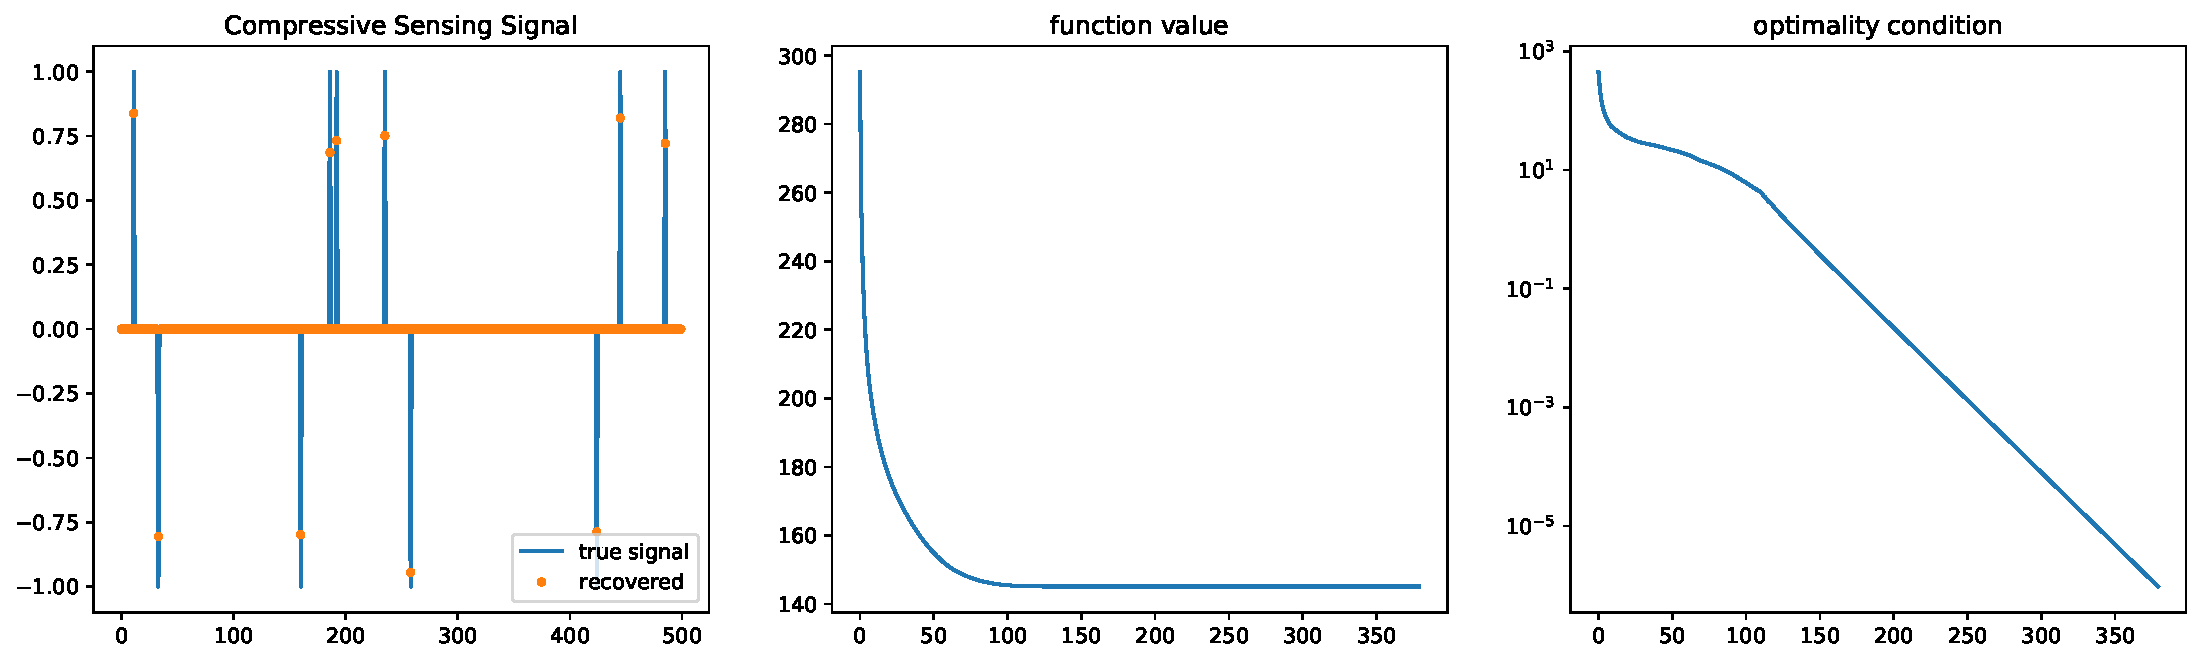
\includegraphics[width=\textwidth]{img/cs_pgd.pdf}
        \caption{Proximal Gradient Descent}
        \label{cs_pgd}
    \end{figure}
    
\item[(c)] Accelerated proximal gradient decent requires fewer iterations to terminate with the default condition.
        \begin{figure}[ht]\centering
            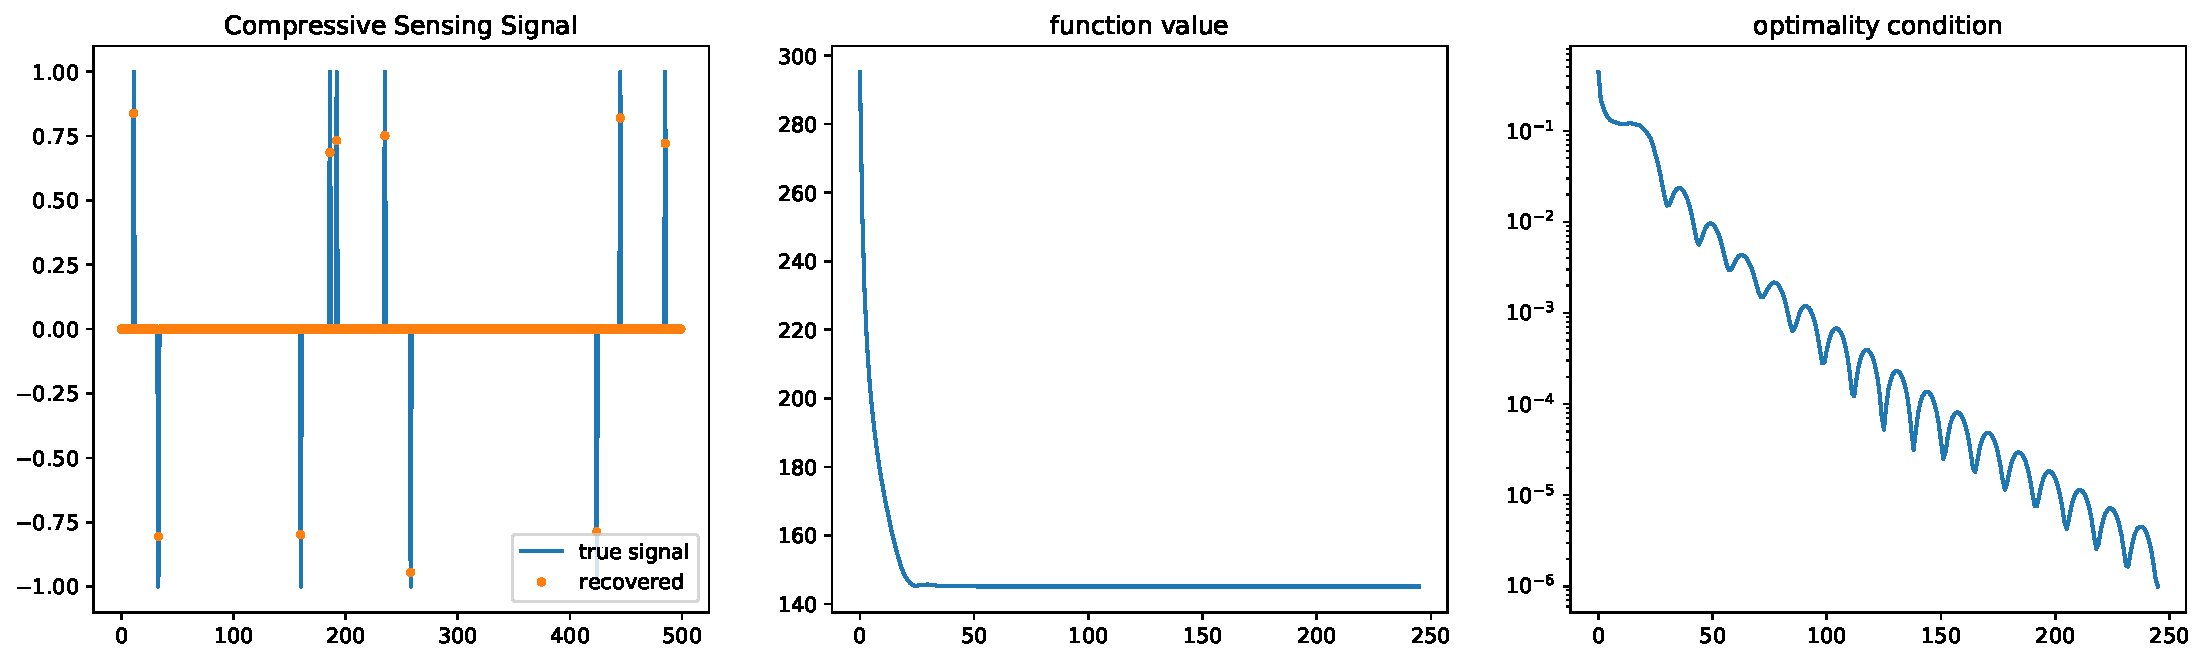
\includegraphics[width=\textwidth]{img/cs_apgd.pdf}
            \caption{Accelerated Proximal Gradient Descent}
            \label{cs_apgd}
        \end{figure}
 

\end{enumerate}

\end{solution}

\begin{problem}[Problem 6]
Logistic regression on MNIST data, recall the logistic regression problem,
\[
\min_{x}~~\sum_{i=1}^m \left\{\ln(1 + \exp(\langle a_i, x \rangle)) - b_i \langle a_i, x \rangle \right\} + \frac{\lambda}{2}\|x\|^2.
\]
We will try to use logistic regression to classify the ``0'' and ``1'' images from MNIST.

In this specific example, \( a_i \) is our image (vectorized), and \( b_i \) is the corresponding label.
By solving the above optimization problem, we want to obtain an classifier, so that for a new image \( a_\text{new} \), we could say
\[\begin{cases}
a_\text{new} \text{ is a 0}, &\text{if } \langle a_\text{new}, x \rangle \le 0\\
a_\text{new} \text{ is a 1}, &\text{if } \langle a_\text{new}, x \rangle > 0
\end{cases}.\]

\begin{enumerate}[label=(\alph*)]
\item[(a)] Complete the function, gradient and Hessian for the logistic regression.
\item[(b)] Apply gradient, accelerate gradient and Newton's method to solve the problem. Which one is the fastest and which one is the slowest?
\item[(c)] What is your accuracy of the classification for the test data.
\end{enumerate}
\end{problem}

\begin{solution}[Solution]
\begin{enumerate}[label=(\alph*)]
    \item[(b)] Figure~\ref{lr} shows the convergence of Gradient Descent, Accelerated Gradient Descent, and Newton's method on a logistic regression problem. We observe Newton's Method requires the fewest iterations.
        
        Both Gradient Decent methods reached the maximum number of iterations without terminating. However, the standard Gradient Descent was worse both in terms of the objective function value and the optimality condition.

        However, iterations may not correspond to ``speed'' since Newton's method requires a linear solve at each iteration.
        \begin{figure}[ht] \centering
            \begin{subfigure}{.9\textwidth}\centering
                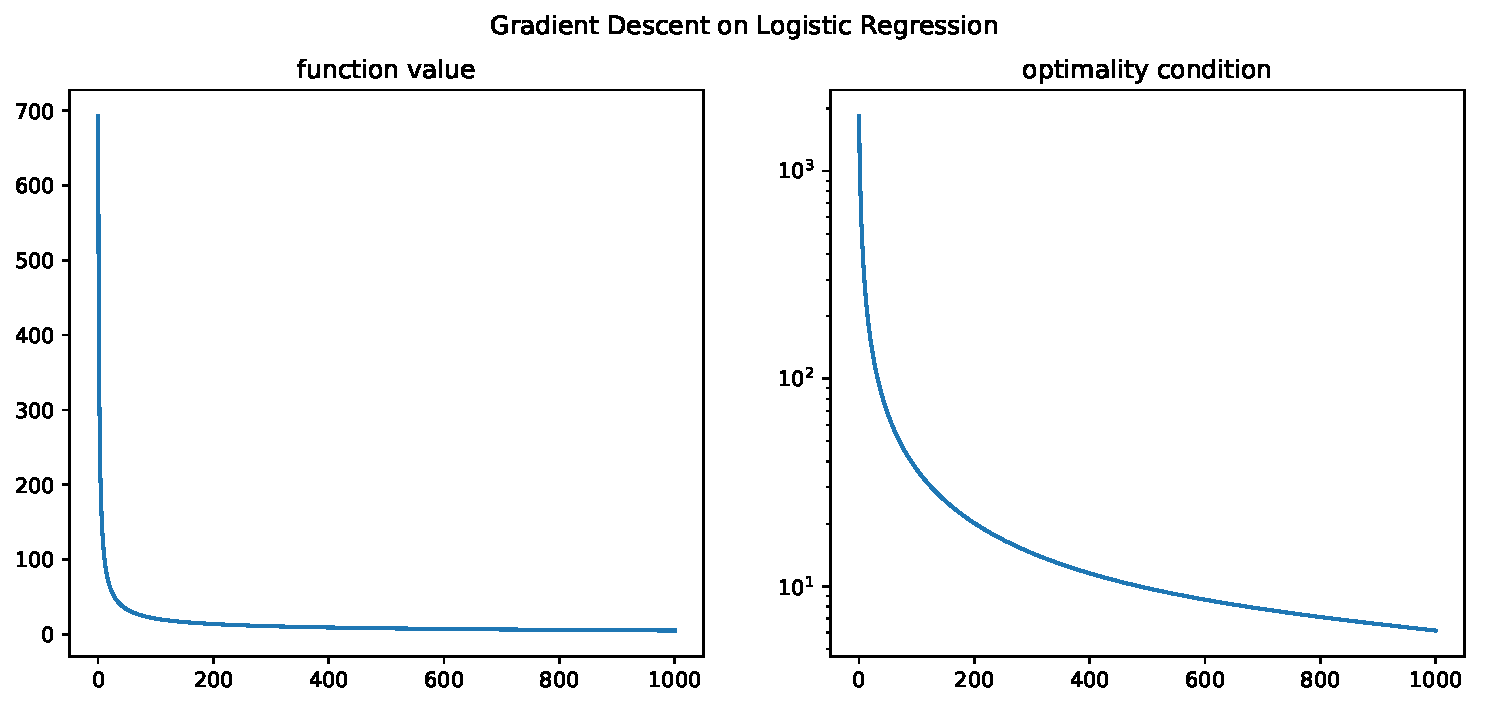
\includegraphics[width=.7\textwidth]{img/lr_gd.pdf}
%                \caption{Gradient Descent}
            \end{subfigure}
            \begin{subfigure}{.9\textwidth}\centering
                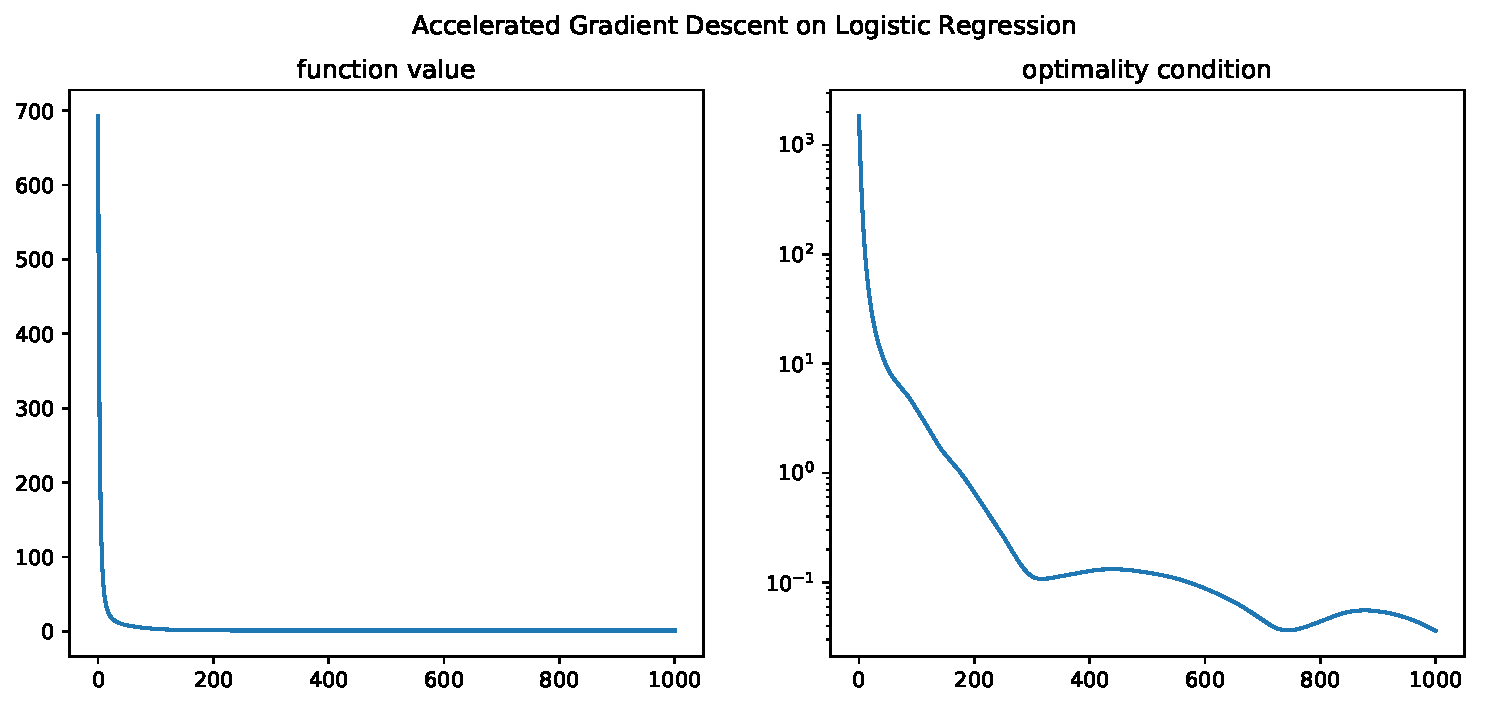
\includegraphics[width=.7\textwidth]{img/lr_agd.pdf}
%                \caption{Accelerated Gradient Descent}
            \end{subfigure}
            \begin{subfigure}{.9\textwidth}\centering
                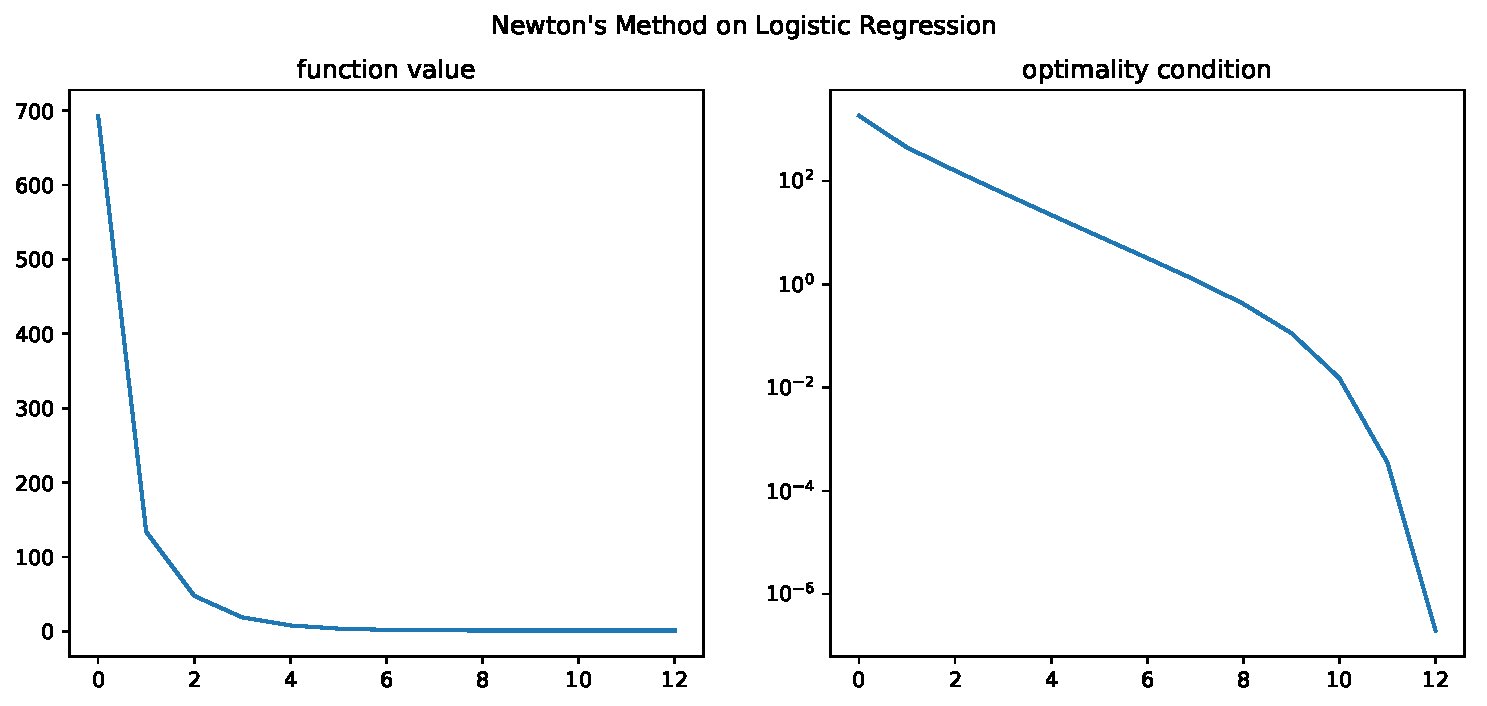
\includegraphics[width=.7\textwidth]{img/lr_nm.pdf}
%                \caption{Newton's Method}
            \end{subfigure}
            \caption{Convergence of Logistic Regression}
            \label{lr}
        \end{figure}
        
    \item[(c)] We have 100\% accuracy.
\end{enumerate}

\end{solution}

\end{document}
